\documentclass[aspectratio=169]{beamer}

%%%%%%%%%%%%
%%% PACKAGES
%%%%%%%%%%%%
\usepackage[T1]{fontenc}
\usepackage[sfdefault,scaled=.85]{FiraSans}
\usepackage{newtxsf}
\usepackage{xcolor}
\usepackage{color}
\usepackage{framed}
\usepackage{graphicx}
\usepackage{amsmath}
\usepackage{multicol}
\usepackage{tikz}
\usepackage{siunitx}
\usepackage{pgfplots}
\usepackage[font={footnotesize}]{caption}
\usepackage{setspace}

%%%%%%%%%%%%%%%%%%
%%% CUSTOMISATIONS
%%%%%%%%%%%%%%%%%%
\usetikzlibrary{intersections}
\pgfplotsset{compat=1.15}
\baselineskip=25pt
\newcommand{\highlight}[1]{\fcolorbox{yellow}{yellow}{#1}}
\usetheme[progressbar=frametitle, numbering=none]{metropolis}
\definecolor{red}{RGB}{150, 20, 20}
\definecolor{grey}{RGB}{150, 150, 150} % 0 (black) to 255 (white)
\definecolor{faded}{RGB}{215, 215, 215}
\definecolor{ash}{RGB}{184, 184, 184}
\setbeamercolor{background canvas}{bg=white}
\setbeamercolor{frametitle}{bg=white, fg=red}
\setbeamercolor{progress bar}{fg=red,bg=faded}

% must add equation numbers in Part 1.
% rewrite sections.
% A better chronological description for blackbody.
% bit of part 2 and 3 are unfinished.
% some statements needs to be rechecked.

\title{Understanding the spectrum of a blackbody}
\institute{\color{grey} Guided by V.H. Belvadi \\ Dept. of Physics \\ Yuvaraja's College, Mysuru}
\author{Sudheendra B.R. \\ Suhas P.K. \\ Shahsank K.K.}
\date{\vspace*{1ex}\color{grey}{\footnotesize March 2020}}

\begin{document}

\begin{frame}[noframenumbering]
	\titlepage
\end{frame}

\begin{frame}[noframenumbering]{Overview}
	\begin{multicols}{2}
		\tableofcontents[sections={1}]
		
			\columnbreak
			
		\tableofcontents[sections={2}]	
	\end{multicols}
	
\end{frame}
\begin{frame}[noframenumbering]{Overview}
	\tableofcontents[sections={3}] 
\end{frame}

\metroset{numbering = counter}

\section{\textbf{Part 1}}

\subsection{The Black Body problem}

\begin{frame}{Introduction}

{\centering
\setstretch{1.5}
{\Large An idealised object that can \textbf{absorb}, and subsequently \textbf{emit}, all the radiation incident on it is called a \highlight{blackbody}.}

}

\end{frame}

\subsection{Charged oscillators} %this section is not needed, i guess
 
\subsection{Rayleigh's intensity function}

\begin{frame}{Rayleigh's law}

	\begin{multicols}{2}
	
	
		\includegraphics[scale=0.28]{unboxed.jpg} \pause
	 
 
		\columnbreak
		
		\begin{itemize}
		
			\item Consider gaseous medium, in which we have a charged oscilator (Say an electron). \pause \newline
			\item Due to random motion of the gaseous atoms, it often collides with the oscillator. \pause \newline
			\item As a result the gaseous atoms imparts some of it's kinetic energy to the oscillator.
		
		\end{itemize}

	
	\end{multicols}
		

\end{frame}

\begin{frame}{Rayleigh's law}
	
		\begin{itemize}
			
		\item {\large Kinetic energy of the oscillator is, $\frac{1}{2}\,kT$.} \newline
		 
		\item {\large And the total kinetic energy will be  $ kT $. }
		 
		\end{itemize}
		
\end{frame}
	
\begin{frame}{Rayleigh's law}

	 	
		\begin{multicols}{2}
  			\begin{itemize}
  				\item {\large Since the charge is radiating energy \textbf{the system cannot attain equilibrium}} \pause
  			\end{itemize}
  				
	\columnbreak
	
			\includegraphics[scale=.28]{boxed.jpg}
			
		\end{multicols}
		

	
\end{frame}
	
\begin{frame}{Rayleigh's law}

	 	
		\begin{multicols}{2} 
		
  			\begin{itemize}
  			
  				\item {\large Since the charge is radiating energy \textbf{the system cannot attain equilibrium}}
  				\item {\large Inner walls of the box is totally reflective.}
  				
  			\end{itemize}
  				
 	
	\columnbreak
	
			\includegraphics[scale=.28]{boxed.jpg}
			
		\end{multicols}
		

	
\end{frame}
		
\begin{frame}{Rayleigh's law}
		
		So, the energy radiated  by the oscillator  per second can be given by, \newline
		{\large \[ \frac{1}{Q} = \frac{\left(\frac{dW}{dt}\right)}{\omega_0 W}\]}\newline
			{\small $Q$ is the radiation reaction. \\ $\omega_0$ is the natural frequency of vibration. \\ $W$ is the total energy content of the oscillator.} 
				
\end{frame}
	
		
\begin{frame}{Rayleigh's law}
		Also, we have 
		\[ \frac{1}{Q}= \frac{\gamma}{\omega_0} \]
			
			\begin{center}		
				{\small Where $\gamma$ is the dampping constant.}
			\end{center}
			
		
\end{frame}


\begin{frame}{Rayleigh's law}

	 \begin{center}
	 
	 	{\large Average energy loss due to radiation is given by,}
	
	 {\large \[ \left<\frac{dW}{dt}\right> = \gamma kT\]}	 
	  {\large Since the degree of freedom is 3,}
	 {\large \[ \left<\frac{dW}{dt}\right> = 3 \gamma kT\]}
	  \end{center} 
\end{frame}
		
\begin{frame}{Rayleigh's law}
	
	\begin{itemize}
		
		\item  $ \mathbf{I}(\omega)d\omega $ is the incident light energy within a frequeny range $d\omega$. \newline
		\item \textbf{Asumption:} The radiation which falls on a \textit{cross section} '$\sigma_s$' is absorbed completely, \newline
		\item Scattered light is the product of $ \mathbf{I}(\omega)d\omega $ and $ \sigma_s $.

	\end{itemize}
	
\end{frame}
			
\begin{frame}{Rayleigh's law}
	\begin{center}
		Expression for the cross section is given by,
	\end{center}
	
	{\large \[ \sigma_s = \frac{8\pi {r_0}^{2}}{3} \left[ \frac{\omega^{4}}{(\omega^2-{\omega_0}^{2})^2+\gamma^2 \omega^2}\right] \]}\newline
	When $ \omega\,=\,\omega_0 $, \newline 		
	{\large \[ \sigma_s = \frac{2\pi {r_0}^{2}{3} \omega_0^{2}}{3(\omega-\omega_0)^2+\dfrac{\gamma^2}{4}} \]}
	
\end{frame}
				
\begin{frame}{Rayleigh's law}

	\[ \frac{dW_s}{dt}=\int_0^{\infty}{\mathbf{I}(\omega)\,\sigma_s \, d\omega} = \int_0^{\infty}{\frac{2\pi {r_0}^{2} \omega_0^{2} \, \mathbf{I}(\omega)\, d\omega}{3 \left[ (\omega-\omega_0)^2+\dfrac{\gamma^2}{4} \right] }} \] \newline

	 \because ($\omega =\omega_0 $), 
	\[ \frac{dW_s}{dt}= \frac{2}{3}\pi {r_0}^{2} \omega_0^{2} \, \mathbf{I}(\omega_0) \int_{-\infty}^{\infty}{\frac{d\omega}{(\omega-\omega_0)^2+{\left(  \dfrac{\gamma}{2} \right)}^{2}}}  \]

\end{frame}

\begin{frame}{Rayleigh's law}\vspace{1cm}

	The integral reduces to arctan function. We get, $2\pi / \gamma$. 
		\begin{align*}
			\frac{dW_s}{dt} &= \frac{dW}{dt} = 3 \gamma kT \\[2ex]
			\therefore \mathbf{I}(\omega) &= \frac{9\gamma^2\,kT}{4\pi^2 r_0^2\omega_0^2} \\[2ex]
			\implies \gamma &= \frac{2}{3} \frac{r_0 \omega_0^2}{c}
		\end{align*}
	
\end{frame}

\begin{frame}{Rayleigh's law}

		
		\begin{align*}
		\implies \gamma &= \frac{2}{3} \frac{r_0 \omega_0^2}{c} \\[2ex]
		\end{align*}
			{\large The intensity distribution function $\mathbf{I}(\omega)$ is, }
		\begin{align*}	
	 	\mathbf{I}(\omega) &=\frac{\omega^2\,kT}{\pi^2 c^2} 
		\end{align*}

\end{frame}


				
\subsection{The Ultra-Violet catastropy} 

\begin{frame}[fragile]{The experimental observation}
\vspace*{2ex}
\begin{figure}
	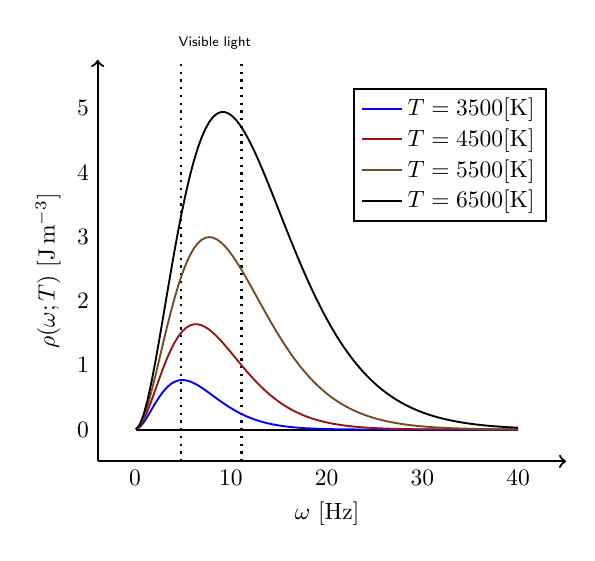
\begin{tikzpicture}[samples=100, scale=0.85]
		\draw[->,thick] {(0,0) -- (0,6)};
		\draw[->,thick] {(0,0) -- (7,0)};
		\draw[dotted,thick] {(1.25,0) -- (1.25,6)};
		\draw[dotted,thick] {(2.15,0) -- (2.15,6)};
		\node at (1.75,6.25) {$\textrm{\textsf{\tiny Visible light}}$};
    \begin{axis}[
        xlabel={$\omega$ [\si{\hertz}]},
        ylabel={$\rho (\omega; T)$ [\si{\joule\per\cubic\meter}]},
        no markers,
        domain=0.1:40,
		  axis line style={draw=none},
		  tick style={draw=none},
        style={thick}]

       \addplot [forget plot,name path=B,samples=2] {0};

    \pgfplotsinvokeforeach{3500, 4500, 5500, 6500}
    {
        \addplot+ 
        {(x^3)/((pi^2)*(exp(2000*x/(#1))-1))};
        \addlegendentryexpanded{$T = #1 [\si{\kelvin}]$}
    }

    \end{axis}
    
    \end{tikzpicture}
\caption{Spectrum of a blackbody.}
\end{figure}

\end{frame}

\subsection{Plank's emphirical formula}

\begin{frame}{}

	\begin{multicols}{2}
	
\begin{center}

 {\large A theoretical explanation for the obtained experimental results were needed. }

\end{center}
 
	\columnbreak

		\begin{center}	
	
	 		\includegraphics[scale=.15]{Maxplank.jpg}
	 
		\end{center}
	
	\end{multicols}
				
\end{frame}

\begin{frame}{}

	\begin{itemize}

		\item The harmonic oscillator can take up energies only in the multiples of $ \mathbf{\hbar \omega} $.  \newline
		\item The probability of occupying an energy level \textbf{E} is {\large $\mathbf{P(E)} = \alpha e^{-\hbar \omega / kT}$} . 
	\end{itemize}
	
\end{frame}

\begin{frame}

	\begin{itemize}
	
		\item The number of oscillators in ground state is $ N_0 $ . \newline
		\item The number of oscillator in first state is $ N_1 = N_0  e^{-\hbar \omega / kT} $.  \vspace{0.5cm}
		\item Then $ N_n = N_0 x^n $ , where $ x = e^{-\hbar \omega / kT} $
	
	\end{itemize}
	
\end{frame}

\begin{frame}

	\begin{itemize}
	
		\item The energy in the ground state is zero. \newline
		\item The energy in the first state is $ N_1 \hbar \omega $ or $ N_0 \hbar \omega x $ \newline
		\item Total energy is given by \[ E_{\left(total \right)} = N_0 \hbar \omega ( 0 + x + 2 x^2 + \cdots ) \] 
	
	\end{itemize}
	
\end{frame}
\begin{frame}
	\begin{itemize}

		\item The total number of oscillators is \[ N_{\left(total \right)} = N_0 ( 1 + x +  x^2 + \cdots ) \]  \newline
		\item  The average energy is \[ \left< E \right> = \frac{E_{\left(total \right)}}{N_{\left(total \right)}} = \dfrac{N_0 \hbar \omega ( 0 + x + 2 x^2 + \cdots )}{N_0 ( 1 + x + x^2 + \cdots )} \] \newline
		
	\end{itemize}
\end{frame}

\begin{frame}


		 \[ Y = 1 + 2 x + 3 x^2 + \cdots  \] \newline
		\[ Yx = x + 2 x ^ 2 + 3 x^3 + \cdots  \] \newline
		 \[ Y(1-x) = 1 + x + x^2 + \cdots  \]

\end{frame}

\begin{frame}

		\[ Y = \dfrac{1}{(1 - x )^2 } \] \newline
		\[ \left< E \right> = \dfrac{ N_0 \hbar \omega x / (1 - x )^2}{ N_0 / (1 - x )} \] 
\end{frame}

\begin{frame}{}

		\[ \left< E \right> =  \frac{\hbar \omega e^{-\hbar \omega / kT} }{1 - e^{-\hbar \omega / kT} } \hspace {1.5cm} \because x = e^{-\hbar \omega / kT}  \] 
		
		\begin{equation}	
		\boxed{ \left< E \right> = \frac{\hbar \omega}{e^{\hbar \omega / kT}-1} }
		\end{equation}
		
\end{frame}

\begin{frame}
	\begin{center}
		{\large Hence The intensity of radiation for frequency $\omega$ is given by,
			\begin{equation}
			I(\omega)d\omega = \frac{\hbar \omega^3 d\omega}{ \pi^2 c^2 \left(e^{\hbar \omega / kT}-1 \right) } 
			\end{equation}
		}
	\end{center}
\end{frame}

\begin{frame}[fragile]{Graph}
\vspace*{2ex}
\begin{figure}
	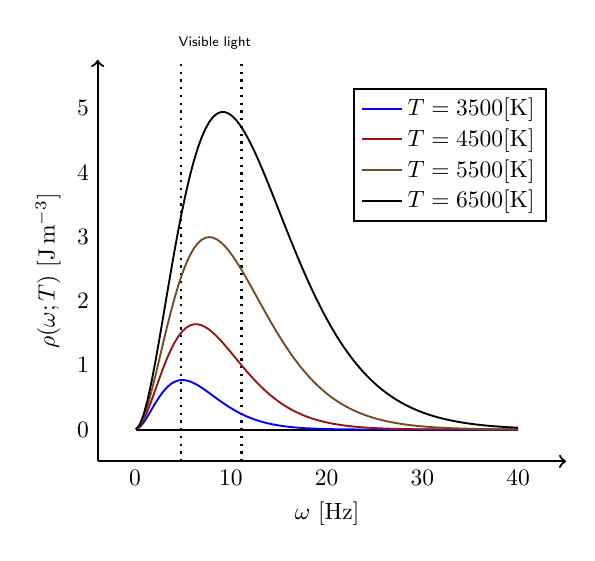
\begin{tikzpicture}[samples=100, scale=0.85]
		\draw[->,thick] {(0,0) -- (0,6)};
		\draw[->,thick] {(0,0) -- (7,0)};
		\draw[dotted,thick] {(1.25,0) -- (1.25,6)};
		\draw[dotted,thick] {(2.15,0) -- (2.15,6)};
		\node at (1.75,6.25) {$\textrm{\textsf{\tiny Visible light}}$};
    \begin{axis}[
        xlabel={$\omega$ [\si{\hertz}]},
        ylabel={$\rho (\omega; T)$ [\si{\joule\per\cubic\meter}]},
        no markers,
        domain=0.1:40,
		  axis line style={draw=none},
		  tick style={draw=none},
        style={thick}]

       \addplot [forget plot,name path=B,samples=2] {0};

    \pgfplotsinvokeforeach{3500, 4500, 5500, 6500}
    {
        \addplot+ 
        {(x^3)/((pi^2)*(exp(2000*x/(#1))-1))};
        \addlegendentryexpanded{$T = #1 [\si{\kelvin}]$}
    }

    \end{axis}
    
    \end{tikzpicture}
\caption{Spectrum of a blackbody.}
\end{figure}

\end{frame}



\section{Part 2}

\subsection{Intensity of a Black Body spectrum and the problem}

\begin{frame}{}

	\begin{itemize}

		\item The intensity of radiation for frequency $\omega$ is given by \[I(\omega)d\omega = \frac{\hbar \omega^3 d\omega}{ \pi^2 c^2 \left(e^{\hbar \omega / kT}-1 \right) } \] \newline
		\item Planck considered that the matter was quantized and not light. \newline
		\item Einstein came up with an alternate idea to solve Black body problem.
		 
	\end{itemize}
	
\end{frame}


\subsection{Einstein's work on Black Bodies}

\begin{frame}{}

	\begin{itemize}

		\item Einstein considered that even the light was quantized, by taking that light is actually photons with energy $\hbar \omega$   \newline
		\begin{center}	
	
	 		\includegraphics[scale=.5]{emission.jpg}
	 
		\end{center}

	\end{itemize}
	
\end{frame}

\begin{frame}{}

	\begin{itemize}
	
		\item Einstein assumed that Planck's formula was right. \newline
		\item Consider two energy levels , say , the $n^{th}$ level and $m^{th}$ level. \newline
	\end{itemize}
	
\end{frame}

\begin{frame}

	\begin{itemize}

		\item The probability of the transition is proportional to intensity of the light. \newline
		
	\end{itemize}
		
			\begin{equation}
					 R_{n \to m} = N_{n} B_{nm} I(\omega) 	 
			\end{equation} 
						
\end{frame}

\begin{frame}{}

	\begin{itemize}

		\item Einstein considers that there are two types of emissions that take place in an atom. \newline
		\item Spontaneous emission. \newline
		\item Stimulated emission.
		
	\end{itemize}
	
\end{frame}

\begin{frame}{}

	\begin{itemize}
	
		\item The combined mathematical expression is,
		
	\end{itemize}
	
			\begin{equation}
					 R_{m \to n} = N_{m} [A_{mn} + B_{mn} I(\omega)] 
			\end{equation} 
	
\end{frame}

\begin{frame}{}

	\begin{itemize}

		\item At thermal equilibrium, the number of atoms going to higher energy level ,ust be equal to the number of atoms coming to 					  lower energy state. \newline	
		\item The ratio of $ N_{m} $ to $ N_{n} $ is given by $ e^{-\hbar \omega / kT} $  \newline
 
	\end{itemize}
	
\end{frame}

\begin{frame}{}

	\begin{itemize}

		\item At thermal equilibrium both $ R_{n \to m} $ and $ R_{m \to n} $ are equal.  \newline
		\item $ N_{n} B_{nm} I(\omega) = N_{m} [A_{mn} + B_{mn} I(\omega)] $ \newline
		\item On dividing the previous equation by $ N_{m} $ we get, 
		
	\end{itemize}
	
\end{frame}

\begin{frame}{}

	\begin{itemize}

		\item $ B_{nm} I(\omega) e^{\hbar \omega /kT} = A_{mn} + B_{mn} I(\omega) $ \newline
		\item The equation that Einsteim got for the intensity of radiation for frequency is 
		
	\end{itemize}
	
		\begin{equation}
				 I(\omega) = \frac{A_{mn}}{B_{nm} e^{\hbar \omega / kT} - B_{mn} }	 
		\end{equation}
		
\end{frame}

\begin{frame}{}

	\begin{itemize}

		\item Since Einstein considered that the formula given by Planck was correct, we should get , \newline
		\item  $ B_{nm} = B_{mn} $  and also
		
			\begin{flushleft}
			
				 \[\frac{A_{mn}}{B_{nm}} = \frac{\hbar \omega^3 d\omega}{ \pi^2 c^2} \] 

			\end{flushleft}
			
	\end{itemize}
	
\end{frame}

\begin{frame}{}

	{\Large This is how Einstein rederived Planck's formula from a quantum mechanical viewpoint.}
		
\end{frame}

\section{\textbf{Part 3}}

\begin{frame}{}

	\begin{itemize}

		\item \textbf{P} = probability\newline
		\item $ \phi $ = Probability amplitude \newline
		\item \textbf{P} = $ \,\Bigr\rvert\,\phi \,\Bigr\rvert\,^{2} $ 
		
	\end{itemize}
	
\end{frame}

\begin{frame}{}

	\begin{itemize}

		\item $ \phi $ = $ \phi_{1} + \phi_{2} $ \newline
		\item \textbf{P} = $ \,\Bigr\rvert\,\phi_{1} + \phi_{2} \,\Bigr\rvert\,^{2} $ 
	
	\end{itemize}
	
\end{frame}

\begin{frame}

	\begin{multicols}{2}
	
	\begin{center}
	
	\includegraphics[scale=0.25]{detector.jpg} 

	\end{center}
 
	\columnbreak
	

\begin{center}

\includegraphics[scale=0.25]{detectorA.jpg}

\end{center}

	\end{multicols}


\end{frame}


\begin{frame}{}

	\begin{itemize}
		\item Detector $ 1 $ is set to detect only $ \alpha $ particles and Dectector  $ 2 $ is set to detect only oxygen atoms.\newline
		\item Probability amplitude of the scattering is given by $ f(\theta)$ when they are at an angle $\theta$.\newline
		\item The probability of this event = $ \,\Bigr\rvert\,f(\theta) \,\Bigr\rvert\,^{2} $
	\end{itemize}
		
\end{frame}


\begin{frame}{}

	\begin{itemize}
	
		\item Set up the dectectors such that the detectors would dectect either $\alpha$ particle or oxygen atom.\newline
		\item We will not distinguish which particle is which entering the detector.\newline
		\item This means that if oxygen atom in position $\theta$ , then
		$\alpha$ particle on the opposite side is at an angle $\pi-\theta$.
		
	\end{itemize}
	
\end{frame}

\begin{frame}

	\begin{itemize}
	
		\item Probability amplitude of oxygen atom = $f(\pi-\theta)$ \newline
		\item Probability amplitude of $\alpha$ particle = $f(\theta)$ \newline
		\item The probability of a particle 
		being detected at detector 1 = $ \,\Bigr\rvert\,f(\theta) \,\Bigr\rvert\,^{2} $ + $ \,\Bigr\rvert\,f(\pi - \theta) \,\Bigr\rvert\,^{2} $
		
 	\end{itemize}
 	
\end{frame}

\begin{frame}{}

	\begin{itemize}

\item Consider if both are $ \alpha $ particles, \newline
\item Then we would not know which particle entered the detector, so the total probability changes to,  \newline
\item  The probability of a $ \alpha $ particle 
		being detected at detector 1 = $ \,\Bigr\rvert\,f(\theta) + f(\pi - \theta) \,\Bigr\rvert\,^{2} $
		
	\end{itemize}
	
\end{frame}

\begin{frame}

	\begin{itemize}

		\item If  $\theta = \dfrac{\pi}{2}$,  then applying this to the expression  $\,\Bigr\rvert\,f(\theta)+f(\pi-\theta)\,\Bigr\rvert\,^{2}$ we get, \newline
		\item Probability = $4 \,\Bigr\rvert\,f\left(\dfrac{\pi}{2}\right) \,\Bigr\rvert\,^{2}$ , if the particles are indistinguishible.
		
	\end{itemize}
	
\end{frame}

\begin{frame}{}

	\begin{itemize}

		\item Suppose the particles were distinguishible, then the probability for $\theta = \dfrac{\pi}{2}$ when applied for $ \,\Bigr\rvert\,f(\theta) \,\Bigr\rvert\,^{2} $ + $ \,\Bigr\rvert\,f(\pi - \theta) \,\Bigr\rvert\,^{2} $ is given by, \newline
		\item Probability = $2 \,\Bigr\rvert\, f\left(\dfrac{\pi}{2}\right) \,\Bigr\rvert ^{2}$ \newline 
		\item This shows that the probability gets doubled for indistinguishible particles.

	\end{itemize}
	
\end{frame}

\begin{frame}
	\begin{itemize}
		\item \textit{Can we apply the same logic to the electron-electron scattering ? }\newline
		\item \textit{OBSERVATION} : " When we have situation in which the identity of the electron which is arriving at a point is echanged with another one , the new amplitude interfere with old one with an opposite phase." \newline
		\item In electrons case , the interfering amplitude for exchange interfere with a negative sign. \newline
		Probability for electron = $\,\Bigr\rvert\,f(\theta)-f(\pi-\theta)\,\Bigr\rvert\,^{2}$
		 \end{itemize}
\end{frame}

\begin{frame}
 \center \includegraphics[scale=0.25]{table.jpg}
	
\end{frame}

\begin{frame}
	\frametitle{Identical Particles}
	
		{\large \textbf{Identical particles}\,, also called \textbf{indistinguishable particle}\,, are particles that cannot be distinguished from one another.}
		
\end{frame}

\begin{frame}{Identical - Indistinguishable Particles}
	\begin{itemize}
		\item Consider particle 'a' and particle 'b'. \newline
		\item Let the two particle collide and get sacttered in two different directions say '1' and '2' over a surface element $ds_{1}$ and $ds_{2}$ of the detector respectively. \newline
		\item If the particles are indistinguishable then the amplitudes of these process will add up. \newline
		\item Probability that the two particles arrive at $ds_{1}$ and $ds_{2}$ is \newline
		$\,\Bigr\rvert\,<1|a><2|b> + <2|a><1|b>\,\Bigr\rvert\,^{2} ds_{1} ds_{2}$
		
	\end{itemize}
\end{frame}

\begin{frame}
	\begin{itemize}
		\item Integrating over the area of the detector ,  if we let $ds_{1}$ and $ds_{2}$ range over the whole area $(\vartriangle S)$ , we could count each part of the area twice since the expression $\,\Bigr\rvert\,<1|a><2|b> + <2|a><1|b>\,\Bigr\rvert\,^{2} ds_{1} ds_{2}$ contains everything that can happen with any pair of surface elements $ds_{1}$ and $ds_{2}$. \newline
		\item $ Probability_{BOSE} = \dfrac{ \left(4\,\Bigr\rvert a \,\Bigr\rvert^{2} \,\Bigr\rvert b \,\Bigr\rvert^{2}\right)}{2} \left(\vartriangle S\right)$ \newline
		\item This is just twice what we got the probability for distinguished particles. 

	\end{itemize}
\end{frame}

\begin{frame}{State with n Bose particle}
	\begin{itemize}
		\item Consider n particles say a, b, c... scattered in n direction say 1, 2, 3 ... \newline
		\item Probability that each particle acting alone would go into an element of the surface ds of the detector is $\,\Bigr\rvert < >\,\Bigr\rvert^{2} ds$. 
	\end{itemize}
\end{frame} 

\begin{frame}
	\begin{itemize}
		\item \textbf{Assumption} :All particles are distinguishable. \newline
		\item Probability that n particles will be counted together in n different surface elements = $\,\Bigr\rvert a_{1}b_{2}c_{3}... \,\Bigr\rvert^{2}ds_{1}ds_{2}...$ \newline
		\item If the amplitude does not depend on where ds is located in the detector , then the \newline
		$Probability = \left(\,\Bigr\rvert a \,\Bigr\rvert^{2}\,\Bigr\rvert b \,\Bigr\rvert^{2}...\right)(ds_{1}ds_{2}...)$
	\end{itemize}
\end{frame} 

\begin{frame}
	\begin{itemize}
		\item Integrating each dS over the surface $\vartriangle S$ of the dectector \newline 
		$(P_{n})_{different} = \left(\,\Bigr\rvert a \,\Bigr\rvert^{2}\,\Bigr\rvert b \,\Bigr\rvert^{2}...\right)(\vartriangle S)^{n}$ \newline
		\item Now suppose that all the particle are Bose particles.
		\item For n particles, there are n! different , but indistinguishable  possibilities for which we must add the amplitudes. \newline
	\end{itemize}
\end{frame}

\begin{frame}
	\begin{itemize}
	\item Probability that n particles will be counted on the n surface elements is given by \newline $Probability = \left(\,\Bigr\rvert a_{1}b_{2}c_{3}... + a_{1}b_{3}c_{2}... \,\Bigr\rvert^{2}\right)(ds_{1}ds_{2}...)$
	\item $Probability = \left(\,\Bigr\rvert n!abc... \,\Bigr\rvert^{2}\right)(ds_{1}ds_{2}...)$
	\item Integrate each ds over the area $\vartriangle S$ of the detector \newline
	$(P_{n})_{BOSE} = n!\left(\,\Bigr\rvert abc... \,\Bigr\rvert^{2}\right)(\vartriangle S)^{n}$
	\end{itemize}
\end{frame}

\begin{frame}
	\begin{itemize}
	\item Comparing the probability when the particles are distinguishable and indistinguishable \newline
	$(P_{n})_{BOSE} = n!\left(\,\Bigr\rvert abc... \,\Bigr\rvert^{2}\right)(\vartriangle S)^{n}$ \newline
	$(P_{n})_{different} = \left(\,\Bigr\rvert a \,\Bigr\rvert^{2}\,\Bigr\rvert b \,\Bigr\rvert^{2}...\right)(\vartriangle S)^{n}$ 
	\item $(P_{n})_{BOSE} = n!(P_{n})_{different}$
	\end{itemize}
\end{frame}

\begin{frame}
	\begin{itemize}
		\item What is the probability that a Bose particle will go into particular state when there are already n particles present ?
	\end{itemize}
\end{frame}

\begin{frame}{Emission and Absorption of photons}
	\begin{itemize}
		\item When the light is emitted, a photon is "created".\newline
		\item Consider that there are some atom emitting n photons. \newline
		\item \textit{OBSERVATION} : The probability that an atom will wmit a photon into a particular final state is increased by the factor (n+1) if there are already n photons in that state.
	\end{itemize}
\end{frame}

\begin{frame}
	\begin{itemize}
		\item In quantum mechanics we can show that \newline 
		$<\chi|\phi> = <\phi|\chi>^{*}$ \newline
		\item The amplitude to get from any condition $\phi$ to any other condition $\chi$. \newline
		\item We have that amplitude that a photon will be added to some state, say j, when there are already n photons present we can express this conditon as \newline
		$<n+1|n>=(\sqrt{n+1})a$\newline
		$<n|n+1>=\left(\sqrt{n+1}\right)a^{*}$ \newline
		where $a = <j|a>$ is the amplitude when there are no other photons are present.
	
	\end{itemize}
\end{frame}

\begin{frame}
	\begin{itemize}
		\item The amplitude to absorb a phot when there are n photons present is given by \newline
		$<n-1|n> = (\sqrt{n})a^{*}$ \newline
		\item  $<n+1|n>=(\sqrt{n+1})a$\newline
		$<n|n+1>=\left(\sqrt{n+1}\right)a^{*}$ \newline
		\item The above two equation shows that they are symmetric in nature.
	\end{itemize}
\end{frame}

\begin{frame}
	\begin{itemize}
		\item \textit{Thought Experiment}: Lets us consider that there are n photons that are created in the same state, that of same frequency but they cannot be distinguished .\newline
		\item The probability that an atom can emit another poton into same state is \newline
		$(Probability)_{emit} = (n+1)\,\Bigr\rvert\,a \,\Bigr\rvert\,^{2}$  \newline
		\item The probability that an atom absorbs a photon into the same state is \newline
		$(Probability)_{absorb} = (n)\,\Bigr\rvert\, a\,\Bigr\rvert\,^{2}$
	\end{itemize}
\end{frame}

\begin{frame}
	\begin{itemize}
		\item Rate at which an atom will make a transition to downwards has two parts.\newline
		\item Probability that it will make a spontaneous transition $\,\Bigr\rvert\,a\,\Bigr\rvert\,^{2}$  is proportional to the number of photons. \newline
		\item The co-efficient of absorption, of induced emission and spontaneous emission are all equal and are related to the probability of spontaneous emission.
	\end{itemize}
\end{frame}

\begin{frame}{The Blackbody Spectrum}
	\begin{itemize}
	 \item For each light frequency $\omega$, there are certain N number of atoms which have two energy states separated, given by the equation $E = \omega\hslash$. \newline
	 \item Let $N_{e}$ and $N_{g}$ be the average numbers of atoms that are in excited state and ground state. \newline
	 \item In thermal equilibrium at temperature T, from statistical mechanics \newline
	 $\frac{N_{e}}{N_{g}} = e^{\left(\dfrac{-\Delta E}{\omega\hslash}\right)}$  \newline
	\item NOTE: Each atom in the ground stae can absorb a photon and go into the excited state and each atom in the excited state can emit a photon and go to the ground state.
	\end{itemize}
\end{frame} 

\begin{frame}
	\begin{itemize}
		\item At equilibrium, the rate of these two process must be equal. \newline
		\item Rate is proportional to the probability of the event and the number of atoms present.\newline
		\item $\overline{n}$ is the average number of photons present in a given state with the frequency $\omega$
	\end{itemize}
\end{frame}

\begin{frame}
	\begin{itemize}
		\item The absorption rate from the state is $N_{g}\overline{n}\,\Bigr\rvert\,a\,\Bigr\rvert\,^{2}$ , and the emission rate into that state is $N_{e}(\overline{n}+1)\,\Bigr\rvert\,a\,\Bigr\rvert\,^{2}$.
		\item At equilibrium  $N_{g}\overline{n}\,\Bigr\rvert\,a\,\Bigr\rvert\,^{2} = N_{e}(\overline{n}+1)\,\Bigr\rvert\,a\,\Bigr\rvert\,^{2}$
	\end{itemize}
\end{frame}

\begin{frame}
	\begin{itemize}
		\item Solving for the average number of photons present in a given state with the frequency $\omega$ \newline
		$\overline{n} = \dfrac{1}{e^{\hslash\omega/k_{B}T - 1}}$ \newline
		\item The energy of each photon is given by $\dfrac{\hslash\omega}{e^{\hslash\omega}/{k_{B}t} - 1}$ \newline
		\item For any harmonic oscillator, the quantum mechanical energy levels are equally spaced with a seperation $\hslash\omega$.
	\end{itemize}
\end{frame}

\begin{frame}
	\begin{itemize}
		\item The energy levels are equally spaced and the $n^{th}$ energy level is the the mean enegry of the oscillator. \newline 
		\center $(E)_{mean} = \dfrac{\hslash\omega}{e^{\hslash\omega}/{k_{B}t} - 1}$ \newline
		\item Considering the bose particle which donot interact with each other, and in that state the whole system of particles behaves (for all quantum mechanical purpose) exactly like an harmonic oscillator. 
	\end{itemize}
\end{frame}

\begin{frame}
	\begin{itemize}
		\item Analysing the Electro-magnetic field in a box, it show the properties of an harmonic oscillation.
		\item Thus, the number of photons in a particular state in a box, can be equated to the number of energy levels associated with the particular modes of oscillation of the electromagetic fields. 
	\end{itemize}
\end{frame}

\begin{frame}
	\begin{itemize}
		\item Mean energy in any particular modes in a box at a temperature T is given by  \newline
		\center $(E)_{mean} = \dfrac{\hslash\omega}{e^{\hslash\omega}/{k_{B}t} - 1}$\newline
	\end{itemize}
\end{frame} 


\begin{frame}
\textit{ASSUMPTIONS}
	\begin{itemize}
		
		\item For every mode there are some atoms in the box, which have energy levels that can radiate into that mode so that each mode can get into thermal equilibrium.
		\item The assumtion of Blackbody radiation law. 
	\end{itemize}
\end{frame}

\begin{frame}
	\begin{itemize}
		\item There will be billions of modes in the box and there will be many small frequency intervals $\Delta\omega$.
		
	\end{itemize}
	 \center \includegraphics[scale=0.15]{waves.jpg}
\end{frame}

\begin{frame}
	\begin{itemize}
		\item The wave number k is given by $k = \dfrac{t\pi}{\lambda}$.
		\item The $\delta k$ between successive modes is given by \newline
		
			$ \delta k = k_{j+1} - k_{j} = \dfrac{\pi}{L}$\newline
			
		\item An asuumption is made that kL is large that in small interval $\Delta k$, there are many modes. 	
		
		 
	\end{itemize}
\end{frame}

\begin{frame}
	\begin{itemize}
		\item $\Delta W$ is the number of modes in the interval $\Delta k$.\newline
		\item This is given by $\Delta W = \dfrac{\Delta k}{\delta k}$ \newline
		    and $\delta k = \dfrac{j\pi}{L}$.\newline
		    Thus, $ \Delta W = \dfrac{L (\Delta k)}{\pi}$ \newline\newline 
		   \highlight {$ \Delta W = \dfrac{L (\Delta k)}{2\pi}$}
		 
	\end{itemize}
\end{frame}

\begin{frame}
 \center \includegraphics[scale=0.2]{modes.jpg}
\end{frame}

\begin{frame}
	\begin{itemize}
		\item A standing wave in a rectangular box must have an integral number of half waves along each axis.
		\item Thus, $\Delta W$ the number of modes for a vector wave number \textbf{k} between the axes components $k and k+\Delta k$ is \newline
		
		\center $\Delta W = \dfrac{L_{x}L_{y}L_{z}}{(2\pi)^3}(\Delta k_{x}\Delta k_{y} \Delta k_{z})$ \newline
		$dW(K) = V\dfrac{d^3k}{(2\pi)^3}$
		
	\end{itemize}
\end{frame}

\begin{frame}
	\begin{itemize}
		\item Applying the above result to find number of photon modes for photons with frequencies in the range $\Delta k$.
		\item In vaccum the magnitude of \textbf{k} is related to the frequency by \newline
		
		$ \,\Bigr\rvert\,k\,\Bigr\rvert\, = \dfrac{\omega}{c}$.\newline
		\item In the frequency interval $\Delta \omega$, these are all the modes which correspond to k's with magnitude between k and $k + \Delta k$, independent of the direction.
		\item The "volume in the k-space" between k and $k + \Delta k $ is a spherical shell of volume \newline
		$ 4\pi(k^2)\Delta k$.
	\end{itemize}
\end{frame}

\begin{frame}
	\begin{itemize}
		\item The number of modes is then , \newline
		\center $\Delta W = \dfrac{V4\pi(k^2)\Delta k}{(2\pi)^3}$.
		\newline
		\item substitute $k = \dfrac{\omega}{c}$\newline
		
		$ \Delta W(\omega) = \dfrac{V4\pi(\omega^3)\Delta \omega}{(2\pi c )^3}$
		
	\end{itemize}
\end{frame}

\begin{frame}
	\begin{itemize}
	\item These modes are independent, we must for double the number of modes.
	\item This is given by,\newline
	
	$ \Delta W(\omega) = \dfrac{V\pi(\omega^3)\Delta \omega}{(\pi c )^3}$  (for light).
	\end{itemize}
\end{frame}

\begin{frame}
	\begin{itemize}
		\item We have shown that each mode has an average the energy \newline 
		$ \overline{n}\hbar\omega = \dfrac{\hbar\omega}{e^{\hbar\omega/k_{B}T} - 1}$\newline
		\item Multiplying This by the number of modes, we get the energy $\Delta E$ in the modes that lie in the interval $\Delta\omega$ : \newline
		\center $ \Delta E = (\dfrac{\hbar\omega}{e^{\hbar\omega/k_{B}T} - 1})(\dfrac{V\pi(\omega^3)\Delta \omega}{(\pi^2)(c^3)})$  \newline
		
	\end{itemize}
\end{frame}

\begin{frame}
	\begin{itemize}
		\item The photons are the Bose particles,which have tendency to try to get to all into the same state.
	\end{itemize}
\end{frame}


\subsection{Amplitude-based descriptiom of identical particles}

\subsection{n Boson systems}

\subsection{Probability based emission and absorption of Black Bodies}

\begin{frame}{}
	\begin{center}
{\Large Thank you}
	\end{center}
\end{frame}

\end{document}


